\section{Auswertung}

Die in der Auswertung bestimmten Ausgleichsrechnungen werden mit
dem Python Paket \emph{scipy.optimize}\cite{scipy} durchgeführt.
Des Weiteren werden die Fehler und insbesondere die Fehlerfortpflanzungen
mit dem Python Paket \emph{uncertainties}\cite{uncertainties} berechnet.
Die auftretenden logarithmischen Fehler werden, wie folgt berechnet:
\begin{align}
  \label{eq:log_fehler}
  \begin{aligned}
    \sigma\ua{ln,+}(N)&=\ln{\left(N+\sigma\ua{N}\right)}-\ln{N}\\%&
    \sigma\ua{ln,-}(N)&=\ln{\left(N-\sigma\ua{N}\right)}-\ln{N}.
  \end{aligned}
\end{align}
\subsection{Untersuchung der Zerfallskurve von Indium}
Zunächst wird der Nulleffekt der Umgebung gemessen.
Nach einer Zeit von $\SI{900}{\second}$ wurden
\begin{equation*}
  N\ua{indium,null}=167
\end{equation*}
Zerfälle gemessen. Umgerechnet auf $240$ Sekunden ergibt sich:
\begin{equation}
  \label{eq:nulleffekt_indium}
   N\ua{indium,null,240}=\frac{668}{15}.
\end{equation}
Anschließend wird die Aktivität der Indium-Probe untersucht. %-von
Als Resultat ergeben sich die in der Tabelle \ref{tab: indium_messwerte} aufgelisteten Messwerte. %Tabelle
In dieser wurde der Nulleffekt schon berücksichtigt.
\begin{table}
\centering
\caption{Gemessene Anzahl an Zerfällen bei Indium.}
\label{tab: indium_messwerte}
\begin{tabular}{S S S S S }
\toprule
{$t$ in $\si{\second}$} & {Anzahl $N$} & {$\sigma\ua{N}$} & {$\sigma\ua{ln,+}(N)$} & {$\sigma\ua{ln,-}(N)$}  \\
\midrule
 240  & 1914  & 44  & 0.02  & 0.02\\
480  & 1771  & 42  & 0.02  & 0.02\\
720  & 1687  & 41  & 0.02  & 0.02\\
960  & 1665  & 41  & 0.02  & 0.02\\
1200  & 1577  & 40  & 0.02  & 0.03\\
1440  & 1461  & 38  & 0.03  & 0.03\\
1680  & 1491  & 39  & 0.03  & 0.03\\
1920  & 1319  & 36  & 0.03  & 0.03\\
2160  & 1361  & 37  & 0.03  & 0.03\\
2400  & 1233  & 35  & 0.03  & 0.03\\
2640  & 1225  & 35  & 0.03  & 0.03\\
2880  & 1141  & 34  & 0.03  & 0.03\\
3120  & 1062  & 33  & 0.03  & 0.03\\
3360  & 1026  & 32  & 0.03  & 0.03\\
3600  & 948  & 31  & 0.03  & 0.03\\
\bottomrule
\end{tabular}
\end{table}

Die grafische Darstellung ist in Abbildung \ref{fig: plot_indium} zu finden. Bei dieser wurde%zu finden
die Anzahl $N$ logarithmiert, um einen linearen Zusammenhang aufzuzeigen (vgl. \eqref{eq: zerfallsgesetz}).
\begin{figure}
  \centering
  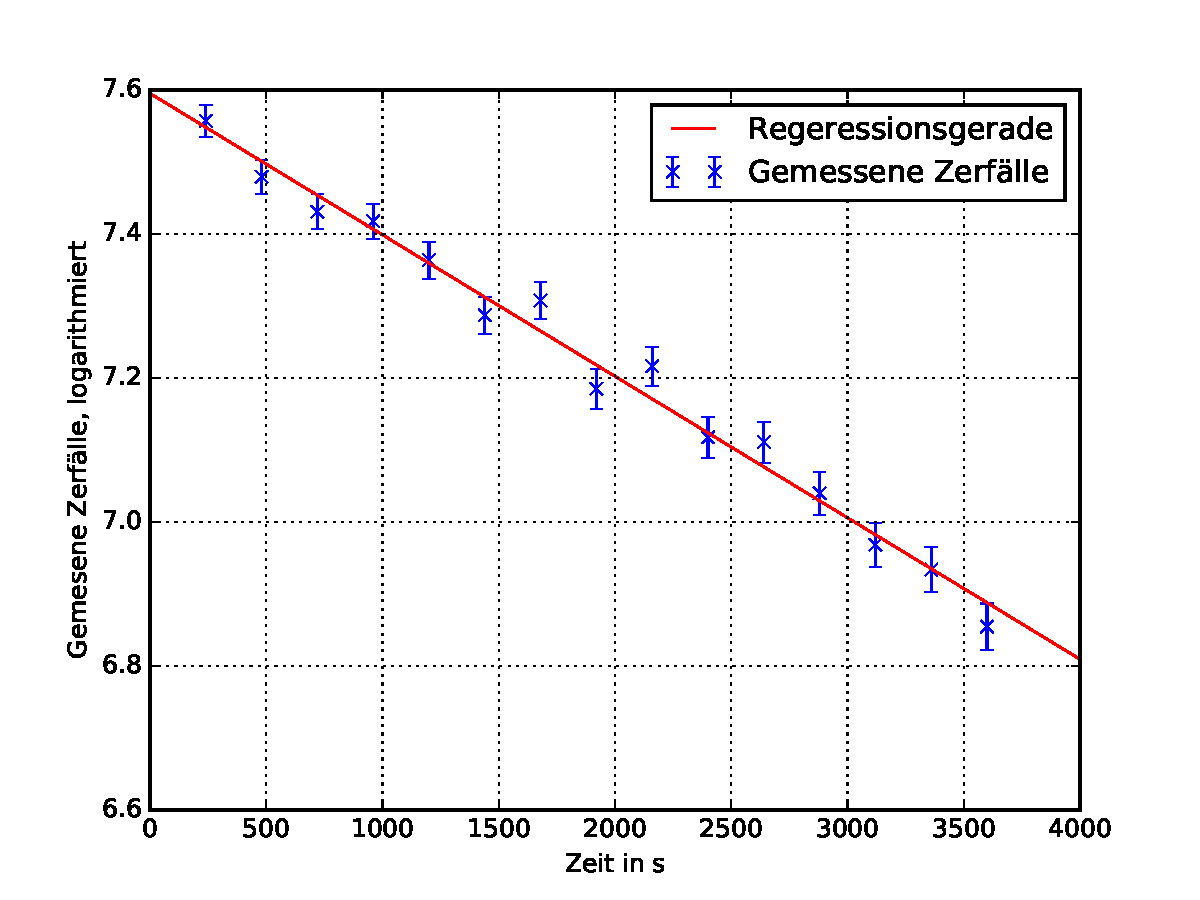
\includegraphics[width=0.8\textwidth]{pics/logarithmiert_indium.pdf}
  \caption{Logarithmierte Darstellung der gemessen Zählraten von Indium und linearer Fit  (unter Berücksichtigung des Nulleffektes).} %Logarithmierte
  \label{fig: plot_indium}
\end{figure}
Der lineare Zusammenhang kann mit Hilfe von
\begin{equation*}
  g(x)=mx+a
\end{equation*}
notiert werden.
Aus der Regressionsrechnung erhält man für die in Abbildung \ref{fig: plot_indium} zu sehende %Abbildung x zu sehende
Ausgleichsgerade die folgenden Parameter:
\begin{align}
  \label{eq:parameter_indium}
  \begin{aligned}
    m\ua{indium}&=\SI{-0.000196\pm0.000007}{\per\second}\\
    a\ua{indium}&=7.595\pm0.015.
  \end{aligned}
\end{align}
Die Parameter aus \eqref{eq:parameter_indium} können in dem direkt Zusammenhang mit
\eqref{eq: n_prozeitintervall} gebracht werden. Und zwar gilt:
\begin{align}
  \label{eq:parameter_indium_vergleich}
  \begin{aligned}
    m\ua{indium}&\Leftrightarrow -\lambda\ua{indium} \quad \Rightarrow \quad \lambda\ua{indium}=\SI{0.000196\pm0.000007}{\per\second}\\
    a\ua{indium}&\Leftrightarrow \ln(b)\ua{indium} \quad \Rightarrow \quad b\ua{indium} =1989\pm 29.
  \end{aligned}
\end{align}
Mit dem Wert für $\lambda\ua{indium}$ und \eqref{eq: halbwertszeit} kann dann die Halbwertszeit von Indium
berechnet weden:
\begin{equation}
  \label{eq:halbwertzeit_indium}
  T\ua{indium}=\SI{3.53\pm0.12 e+3}{\second}.
\end{equation}
Im Gegensatz dazu liegt der Theoriewert für die Halbwertszeit von Indium\cite{indium_halb} bei
\begin{equation}
  \label{eq:halbwertzeit_indium_theo}
  T\ua{indium,theo}=\SI{3.24 e+3}{\second}.
\end{equation}
\subsection{Untersuchung der Zerfallskurve von einem Rhodiumisomer}
Der Nulleffekt, bei der Rhodium Untersuchung beträgt bei $\SI{900}{\second}$
\begin{equation*}
  N\ua{rhodium,null}=218.
\end{equation*}
Umgerechnet auf $15$ Sekunden ergibt sich: %Sekunden
\begin{equation*}
     N\ua{rhodium,null,25}=\frac{109}{30}.
\end{equation*}
Die gemessenen Werte sind in Tabellen \ref{tab: rhodium_messwerte1} und \ref{tab: rhodium_messwerte2} aufgelistet, dabei erfolgte %sind in den Tabellen x und y
der Abzug des Nulleffektes bereits.
\begin{table}
\centering
\caption{Gemessene Anzahl an Zerfällen bei Rhodium}
\label{tab: rhodium_messwerte}
\begin{tabular}{S S S S S }
\toprule
{$t$ in $\si{\second}$} & {Anzahl $N$} & {$\sigma\ua{N}$} & {$\ln{\left(N+\sigma\ua{N}\right)}-\ln{N}$} & {$\ln{\left(N-\sigma\ua{N}\right)}-\ln{N}$}  \\
\midrule
 15.00  & 603.37  & 24.56  & 0.04  & 0.04\\
30.00  & 423.37  & 20.58  & 0.05  & 0.05\\
45.00  & 399.37  & 19.98  & 0.05  & 0.05\\
60.00  & 315.37  & 17.76  & 0.05  & 0.06\\
75.00  & 248.37  & 15.76  & 0.06  & 0.07\\
90.00  & 201.37  & 14.19  & 0.07  & 0.07\\
105.00  & 194.37  & 13.94  & 0.07  & 0.07\\
120.00  & 146.37  & 12.10  & 0.08  & 0.09\\
135.00  & 121.37  & 11.02  & 0.09  & 0.10\\
150.00  & 107.37  & 10.36  & 0.09  & 0.10\\
165.00  & 83.37  & 9.13  & 0.10  & 0.12\\
180.00  & 84.37  & 9.19  & 0.10  & 0.12\\
195.00  & 71.37  & 8.45  & 0.11  & 0.13\\
210.00  & 53.37  & 7.31  & 0.13  & 0.15\\
225.00  & 53.37  & 7.31  & 0.13  & 0.15\\
240.00  & 48.37  & 6.95  & 0.13  & 0.16\\
255.00  & 37.37  & 6.11  & 0.15  & 0.18\\
270.00  & 47.37  & 6.88  & 0.14  & 0.16\\
285.00  & 33.37  & 5.78  & 0.16  & 0.19\\
300.00  & 26.37  & 5.13  & 0.18  & 0.22\\
315.00  & 38.37  & 6.19  & 0.15  & 0.18\\
330.00  & 29.37  & 5.42  & 0.17  & 0.20\\
345.00  & 20.37  & 4.51  & 0.20  & 0.25\\
360.00  & 32.37  & 5.69  & 0.16  & 0.19\\
375.00  & 23.37  & 4.83  & 0.19  & 0.23\\
390.00  & 23.37  & 4.83  & 0.19  & 0.23\\
405.00  & 21.37  & 4.62  & 0.20  & 0.24\\
420.00  & 21.37  & 4.62  & 0.20  & 0.24\\
435.00  & 27.37  & 5.23  & 0.17  & 0.21\\
450.00  & 23.37  & 4.83  & 0.19  & 0.23\\
465.00  & 25.37  & 5.04  & 0.18  & 0.22\\
480.00  & 31.37  & 5.60  & 0.16  & 0.20\\
495.00  & 19.37  & 4.40  & 0.20  & 0.26\\
510.00  & 26.37  & 5.13  & 0.18  & 0.22\\
525.00  & 21.37  & 4.62  & 0.20  & 0.24\\
540.00  & 19.37  & 4.40  & 0.20  & 0.26\\
555.00  & 10.37  & 3.22  & 0.27  & 0.37\\
570.00  & 15.37  & 3.92  & 0.23  & 0.29\\
585.00  & 8.37  & 2.89  & 0.30  & 0.42\\
600.00  & 15.37  & 3.92  & 0.23  & 0.29\\
615.00  & 17.37  & 4.17  & 0.22  & 0.27\\
630.00  & 9.37  & 3.06  & 0.28  & 0.40\\
645.00  & 9.37  & 3.06  & 0.28  & 0.40\\
660.00  & 17.37  & 4.17  & 0.22  & 0.27\\
675.00  & 22.37  & 4.73  & 0.19  & 0.24\\
690.00  & 9.37  & 3.06  & 0.28  & 0.40\\
705.00  & 14.37  & 3.79  & 0.23  & 0.31\\
720.00  & 11.37  & 3.37  & 0.26  & 0.35\\
\bottomrule
\end{tabular}
\end{table}

Die Werte sind in Abbildung \ref{fig: plot_rhodium} dargestellt.
\begin{figure}
  \centering
  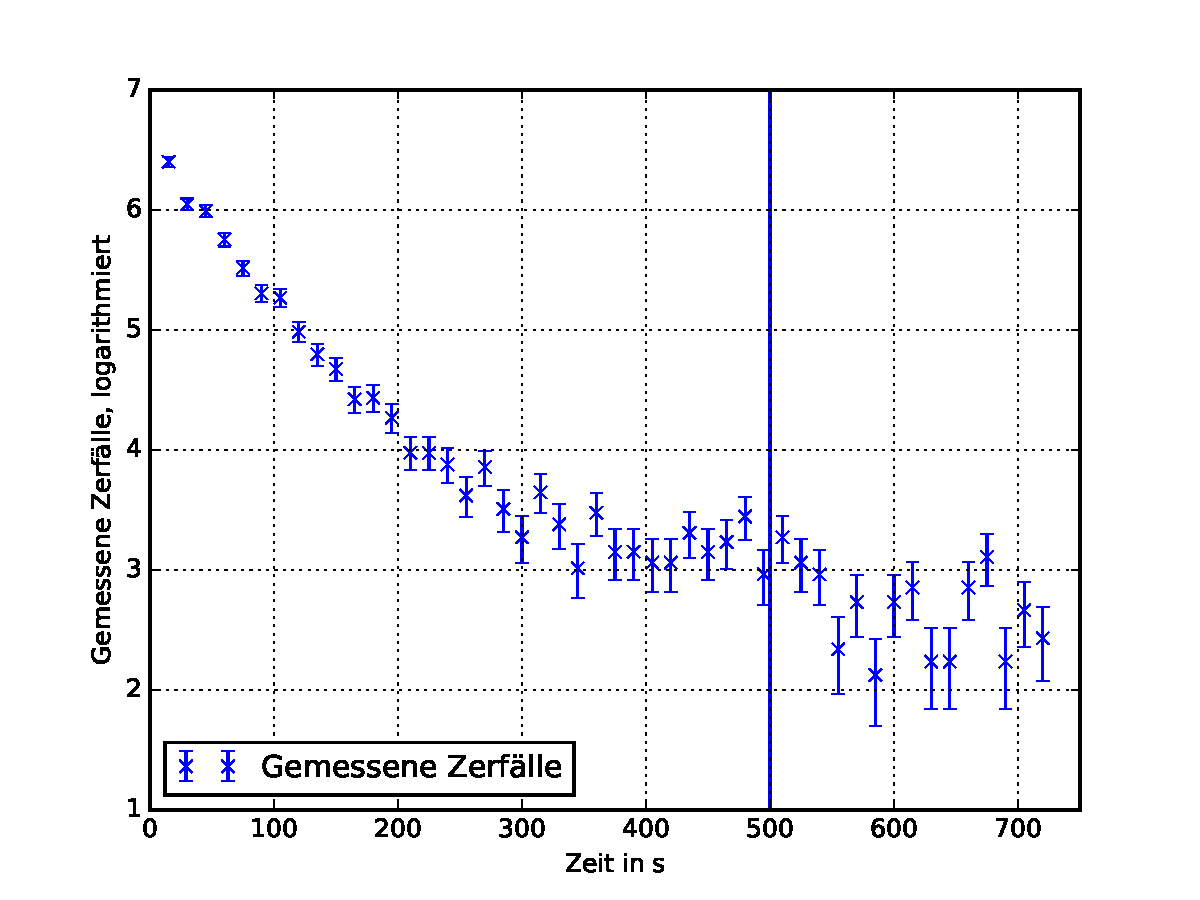
\includegraphics[width=0.8\textwidth]{pics/ra_all.pdf}
  \caption{Logarithmierte Darstellung der gemessen Zählraten von Rhodium (unter Berücksichtigung des Nulleffektes).}
  \label{fig: plot_rhodium}
\end{figure}
Wie in der Theorie erläutert, ist Rhodium ein Isomer aus $\ce{^{104}_{45} Rh}$ (kurzlebig) und %erläutert,
$\ce{^{104i}_{45} Rh}$ (langlebig). Beide Stoffe besitzen eine unterschiedliche Halbwertszeit und
beeinflussen so die in Abbildung \ref{fig: plot_rhodium} dargestellte Aktivitätskurve zu unterschiedlichen
Zeiten.
Ab einer bestimmten Zeit $t*$, wird also nur noch der Zerfall von $\ce{^{104i}_{45} Rh}$
gemessen.
Wir deklarieren $t*=\SI{500}{\second}$ und berechnen dann mit Hilfe einer linearen Regression %-,
die Halbwertszeit von $\ce{^{104i}_{45} Rh}$.
Zusätzlich legen wir eine Zeit $t\ua{kurz}=\SI{150}{\second}$ fest in der
nur der Zerfall von $\ce{^{104}_{45} Rh}$ messbar ist.
\begin{table}
\centering
\caption{Gemessene Anzahl an Zerfällen bei $\ce{^{104}_{45} Rh}$ }
\label{tab:rho_lang_log}
\begin{tabular}{S S S S S}
\toprule
{$t$ in $\si{\second}$} & {Anzahl $N_{\Delta \map{t}, \map{lang}}$} & $\sigma_{\Delta \map{t}, \map{lang}}$ & {$\sigma\ua{ln,+}(N_{\Delta \map{t}, \map{lang}})$} & { $ \sigma\ua{ln,-}(N_{\Delta \map{t}, \map{lang}})$}  \\
\midrule
 510  & 31  & 6  & 0.2  & 0.2\\
525  & 19  & 4  & 0.3  & 0.2\\
540  & 26  & 5  & 0.2  & 0.2\\
555  & 21  & 5  & 0.2  & 0.2\\
570  & 19  & 4  & 0.3  & 0.2\\
585  & 10  & 3  & 0.4  & 0.3\\
600  & 15  & 4  & 0.3  & 0.2\\
615  & 8  & 3  & 0.4  & 0.3\\
630  & 15  & 4  & 0.3  & 0.2\\
645  & 17  & 4  & 0.3  & 0.2\\
660  & 9  & 3  & 0.4  & 0.3\\
675  & 9  & 3  & 0.4  & 0.3\\
690  & 17  & 4  & 0.3  & 0.2\\
705  & 22  & 5  & 0.2  & 0.2\\
720  & 9  & 3  & 0.4  & 0.3\\
\bottomrule
\end{tabular}
\end{table}

Die Messwerte (vgl. Tabelle \ref{tab:rho_lang_log}) und die Regressionsgerade für $t>t*$ sind in \ref{fig: plot_rhodium_lang} abgebildet.
\begin{figure}
  \centering
  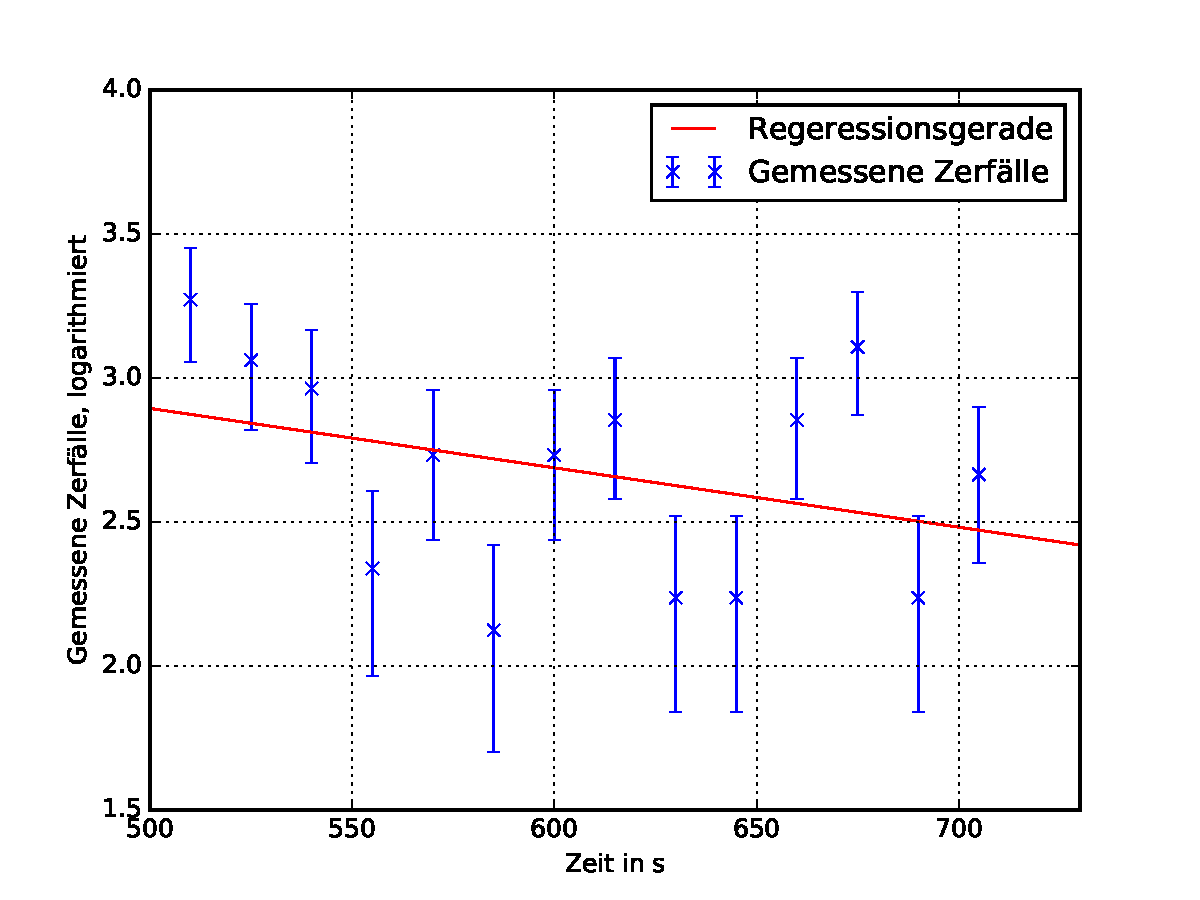
\includegraphics[width=0.8\textwidth]{pics/rhodium_lang_miterror.pdf}
  \caption{Logarithmierte Darstellung der gemessen Zählraten von Rhodium und der lineare Fit, nach $t*$  (unter Berücksichtigung des Nulleffektes).} %Logarithmierte; lineare
  \label{fig: plot_rhodium_lang}
\end{figure}
Die Resultate der Regressionsrechung lauten:
\begin{align}
  \label{eq:parameter_rhodium_lang}
  \begin{aligned}
    m\ua{rho,lang}&=\SI{-0.0021\pm0.0016}{\per\second}\\
    a\ua{rho,lang}&=5.44\pm0.13.
  \end{aligned}
\end{align}
Auch hier herrscht eine Verbindung zu Gleichung \eqref{eq: n_prozeitintervall}:
\begin{align}
  \label{eq:parameter_rhodium_lang_lambda}
  \begin{aligned}
    m\ua{rho,lang}&\Leftrightarrow -\lambda\ua{rho,lang} \quad \Rightarrow \quad \lambda\ua{rho,lang}=\SI{0.0021\pm0.0016}{\per\second}\\
    a\ua{rho,lang}&\Leftrightarrow \ln(b)\ua{rho,lang} \quad \Rightarrow \quad b\ua{rho,lang} =50\pm 50.
  \end{aligned}
\end{align}
Als Halbwertszeit ergibt sich mit \eqref{eq: halbwertszeit}:
\begin{equation}
  \label{eq:halbwertzeit_rhodium}
  T\ua{rhodium, lang}=\SI{3.4\pm2.6 e+2}{\second}.
\end{equation}
Hingegen liegt der Theoriewert\cite{rhodium_lang_halb} bei:
\begin{equation}
  \label{eq:halbwertzeit_rhodium_theo}
  T\ua{rhodium, lang, theo}=\SI{2.6 e+2}{\second}.
\end{equation}
Um die Halbwertszeit von $\ce{^{104}_{45} Rh}$ zu bestimmten, subtrahiert man von der
Gesamtanzahl der Aktivitäten die Zerfallsrate von $\ce{^{104i}_{45} Rh}$ vor dem
Zeitpunkt $t*$:
\begin{equation*}
  N_{\Delta \map{t}, \map{kurz}}(t_i)=N_{\Delta \map{t}, \map{ges}}(t_i)-N_{\Delta \map{t}, \map{lang}}(t_i) \qquad t_i<t*.
\end{equation*}
Die errechneten Werte sind in Tabelle \ref{tab: zerfälle_rhkurz} aufgelistet.
\begin{table}
\centering
\caption{Berechnete Zerfälle von $\ce{^{104i}_{45} Rh}$}
\label{tab: zerfälle_rhkurz}
\begin{tabular}{S S S S S S S }
\toprule
{$t$ in $\si{\second}$} & {Anzahl $N_{\Delta \map{t}, \map{ges}}$} & {$\sigma_{N_{\Delta \map{t}, \map{ges}}}$} & {$N_{\Delta \map{t}, \map{lang}}$} & {$\sigma_{N_{\Delta \map{t}, \map{lang}}}$} &  {$N_{\Delta \map{t}, \map{kurz}}(t_i)$} & {$\sigma_{  N_{\Delta \map{t}, \map{kurz}}}$}   \\
\midrule
 15  & 603  & 25  & 5  & 2  & 598  & 25\\
30  & 423  & 21  & 5  & 2  & 418  & 21\\
45  & 399  & 20  & 5  & 2  & 394  & 20\\
60  & 315  & 18  & 5  & 2  & 310  & 18\\
75  & 248  & 16  & 5  & 2  & 243  & 16\\
90  & 201  & 14  & 5  & 2  & 196  & 14\\
105  & 194  & 14  & 5  & 2  & 189  & 14\\
120  & 146  & 12  & 5  & 2  & 142  & 12\\
135  & 121  & 11  & 5  & 2  & 117  & 11\\
150  & 107  & 10  & 5  & 2  & 103  & 11\\
\bottomrule
\end{tabular}
\end{table}

\begin{table} 
\centering 
\caption{Bestimmte logaritmische Fehler bei $\ce{^{104}_{45} Rh}$  } 
\label{tab:rho_kurz_log} 
\begin{tabular}{S S S S S } 
\toprule  
{$t$ in $\si{\second}$} & {Anzahl $N_{\Delta \map{t}, \map{kurz}}$} & $\sigma_{\Delta \map{t}, \map{kurz}}$ & {$\sigma\ua{ln,+}(N_{\Delta \map{t}, \map{kruz}})$} & { $ \sigma\ua{ln,-}(N_{\Delta \map{t}, \map{kurz}})$}  \\  
\midrule  
 15  & 603  & 25  & 0.04  & 0.04\\ 
30  & 423  & 21  & 0.05  & 0.05\\ 
45  & 399  & 20  & 0.05  & 0.05\\ 
60  & 315  & 18  & 0.06  & 0.06\\ 
75  & 248  & 16  & 0.07  & 0.06\\ 
90  & 201  & 14  & 0.07  & 0.07\\ 
105  & 194  & 14  & 0.08  & 0.07\\ 
120  & 146  & 12  & 0.09  & 0.08\\ 
135  & 121  & 11  & 0.10  & 0.09\\ 
150  & 107  & 10  & 0.10  & 0.09\\ 
\bottomrule 
\end{tabular} 
\end{table}

Zusätzlich findet sich in Abbildung \ref{fig: plot_rhodium_kurz} die grafische Darstellung
und Regeressionsgerade der Messwerte. Die logarithmischen Fehler der Grafik \ref{fig: plot_rhodium_kurz}
sind in Tabelle \ref{tab:rho_kurz_log} zufinden.
\begin{figure}
  \centering
  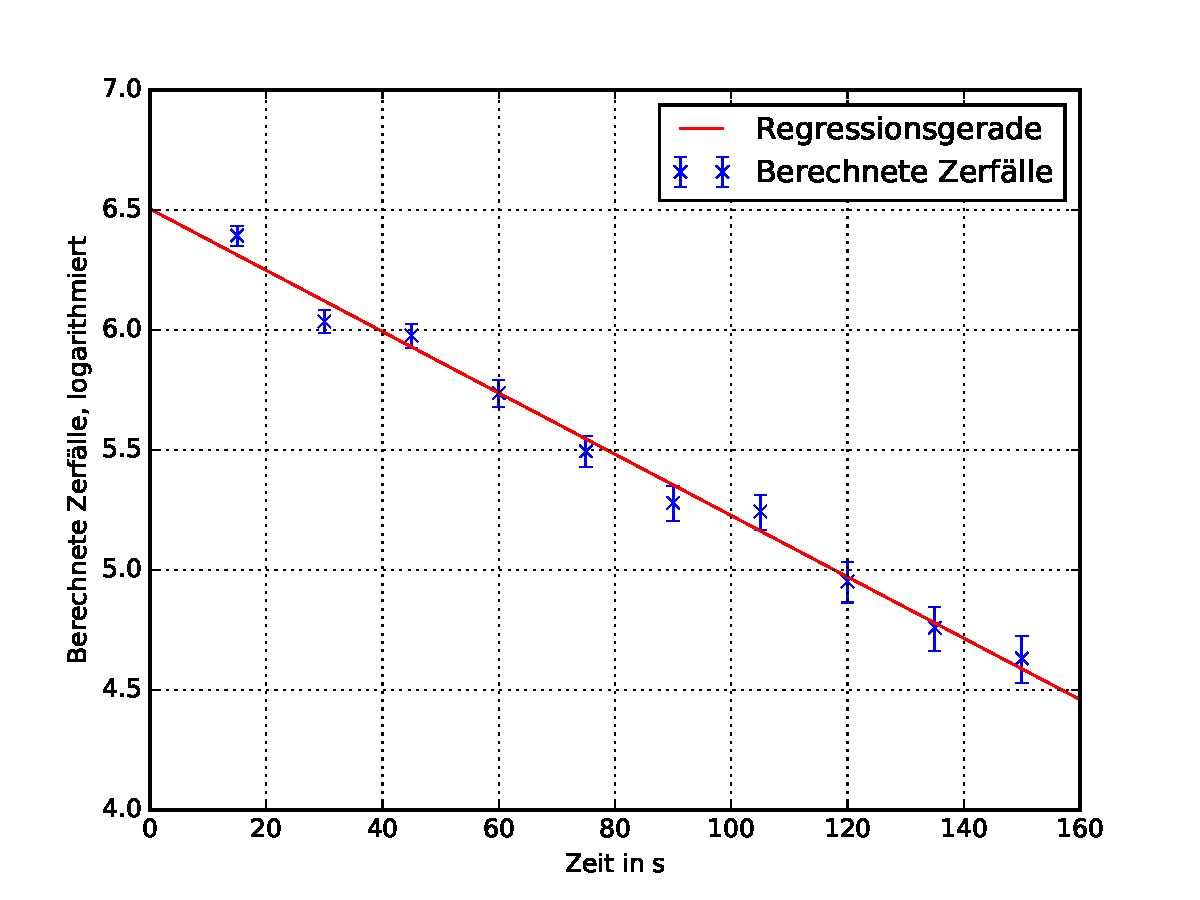
\includegraphics[width=0.8\textwidth]{pics/rhodium_kurz_berechnet.pdf}
  \caption{Logarithmierte Darstellung der berechnete Zählraten von Rhodium $\ce{^{104}_{45} Rh}$ und der linearer Fit, vor $t*$ (unter Berücksichtigung des Nulleffektes).}
  \label{fig: plot_rhodium_kurz}
\end{figure}
Aus der Regressionsrechung erhält man folgende Parameter
\begin{align}
  \label{eq:parameter_rhodium_kurz}
  \begin{aligned}
    m\ua{rho,kurz}&=\SI{-0.0128\pm0.0005}{\per\second}\\
    a\ua{rho,kurz}&=6.50\pm0.04.
  \end{aligned}
\end{align}
Wie bei den vorherigen Parametern kann auf die in \eqref{eq: n_prozeitintervall} auftretenden Größen %-auch; Parametern
geschlossen werden: %geschlossen werden
\begin{align}
  \label{eq:parameter_rhodium_kurz_lambda}
  \begin{aligned}
    m\ua{rho,kurz}&\Leftrightarrow -\lambda\ua{rho,kurz} \quad \Rightarrow \quad \lambda\ua{rho,kurz}=\SI{0.0128\pm0.0005}{\per\second}\\
    a\ua{rho,kurz}&\Leftrightarrow \ln(b)\ua{rho,kurz} \quad \Rightarrow \quad b\ua{rho,kurz} =668\pm 30.
  \end{aligned}
\end{align}
Die Halbwertszeit wird mit \eqref{eq: halbwertszeit} berechnet.
Als Ergebnis erechnet sich:
\begin{equation}
  \label{eq:halbwertzeit_rhodium_kurz}
  T\ua{rhodium, kurz}=\SI{54.3\pm2.0 }{\second}
\end{equation}
Hingegen liegt der Theoriewert\cite{rhodium_kurz_halb} bei:
\begin{equation}
  \label{eq:halbwertzeit_rhodium_kurz_theo}
  T\ua{rhodium, kurz, theo}=\SI{42.3}{\second}.
\end{equation}
Um die Aussagekraft der Resultate zu stützen sollte allgemein gelten:
\begin{equation*}
  N_{\Delta \map{t}, \map{kurz}}(t*)\ll N_{\Delta \map{t}, \map{lang}}(t*).
\end{equation*}
Nach Einsetzten in die Regressionsfunktion ergibt sich jeweils %Einsetzen
\begin{equation*}
    N_{\Delta \map{t}, \map{kurz}}(t*)= 1\pm1 \quad  N_{\Delta \map{t}, \map{lang}}(t*)= 18\pm 4 \quad \Rightarrow \quad N_{\Delta \map{t}, \map{kurz}}(t*)\ll N_{\Delta \map{t}, \map{lang}}(t*).
\end{equation*}
Abschließend werden beide bestimmten Regressionsgeraden ($\eqref{eq:parameter_rhodium_lang}$ und $\eqref{eq:parameter_rhodium_kurz}$) noch addiert, um so eine %-geraden
Regressionsgerade für die Messwerte \ref{tab: rhodium_messwerte1} und \ref{tab: rhodium_messwerte2} zu bilden.
Die sich ergebende Darstellung ist in \ref{fig: plot_rhodium_addi} zu sehen. %zu sehen
\begin{figure}
  \centering
  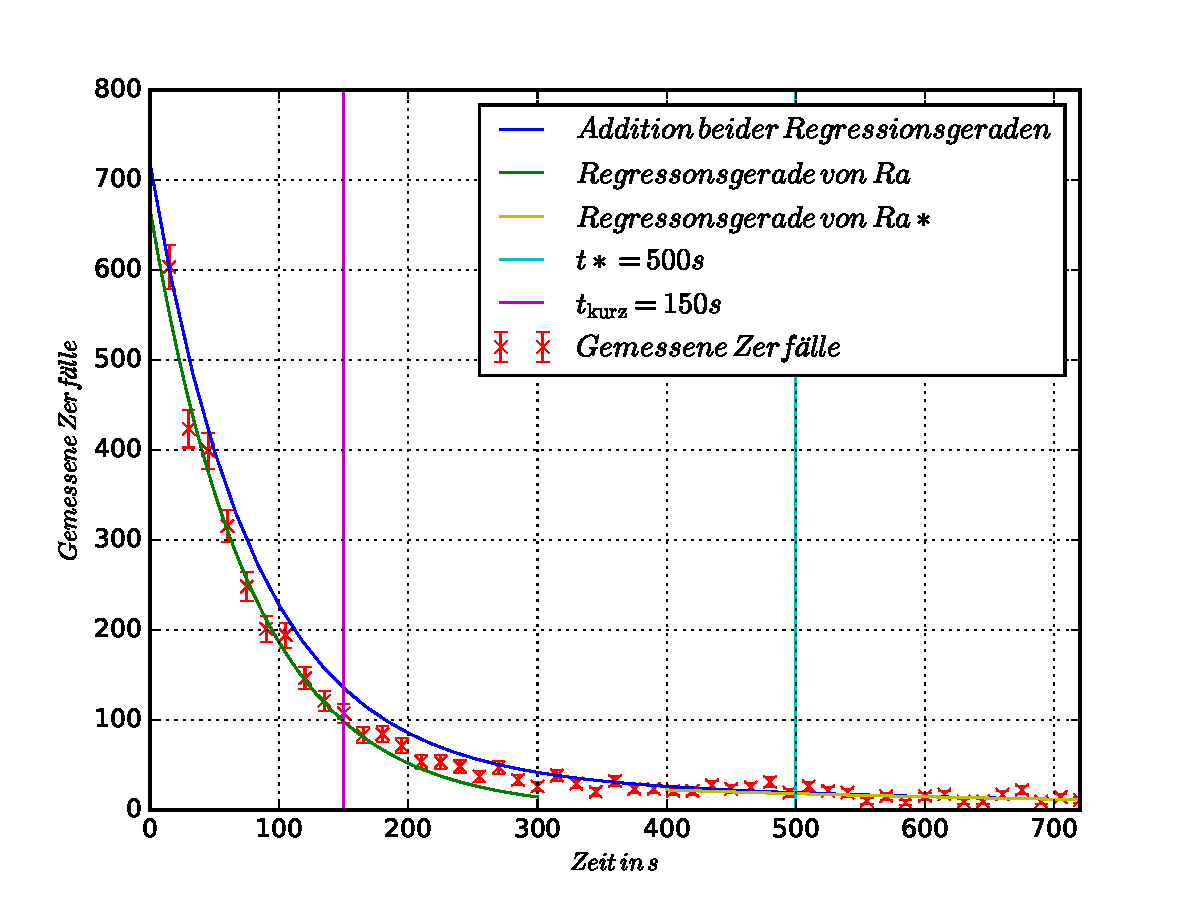
\includegraphics[width=0.8\textwidth]{pics/ra_addi.pdf}
  \caption{Darstellung der berechnete Zählraten von Rhodium mit Regressionskurve, (unter Berücksichtigung des Nulleffektes).} %berechneten
  \label{fig: plot_rhodium_addi}
\end{figure}
